\chapter{\label{chap:state}Bestehende offlinefähige Systeme / Konzepte}

\note{Harte, weiche, mittlere probleme (verschiedene Stufen von offlinefähig)}
\note{Native Apps sind offlinefähig}
bei nativen Apps ist das Problem bei der Datenverteilung
%
% Software
%
\section{Kollaborative Software}
\highlight{rauslassen?}
Kann ich benutzen um kollaborativ zu arbeiten --> \b{was passiert wenn ich offline bin?}
\sub{Google Docs}
(benutzt OT)
\sub{Google Wave}
(benutzt OT)
\sub{Kollaborative Editoren}
Wiki: \url{https://en.wikipedia.org/wiki/Collaborative_real-time_editor}\\\\
\url{https://atom.io/packages/covalent}\\
\url{https://atom.io/packages/firepad}\\
Markdown: \url{https://hackmd.io/}\\
LaTeX: \url{https://www.sharelatex.com/}\\
Online editor: \url{http://etherpad.org/} (OT)\\
Mockingbird (tool for creating wireframes): \url{https://gomockingbird.com/home} (OT)\\
--> Zahl steigend, (nachdem Google die Drive Realtime API veröffentlicht hat, die auf \gls{OT} basiert und es \it{third-party Apps} ermöglicht, dieselbe Zusammenarbeit wie Google Docs zu verwenden)\\\\
\b{plus} wachsende Anzahl von offen zur Verfügung gestellter Bibliotheken und Frameworks die es ermöglichen, offlinefähige Anwendungen zu programmieren. Siehe Kapitel \ref{sec:frameworks}
%
% Frameworks / Bibliotheken
%
\section{\label{sec:frameworks}Offline-First Frameworks/Bibliotheken}
Ich möchte aber auch eigenständig Software entwickeln die man vielleicht nicht nur zum Arbeiten nehmen kann, sondern auch um Quatsch zu machen wie Katzengifs zu teilen.
\Gls{PWAg}
%
% realm
%
\sub{Realm}
Backend für mobile Anwendungen (Java, Swift, C\#, JS). Realm Datenbank oder Realm Platform(= DB+ Object Server).
Schreiben groß `OIffline First Experience` überall hin (webseite, whitepaper...)
\begin{itemize}
  \item lokale DB, plattformübergreifend
  \item Object Server fungiert als Middleware-Komponente in der mobilen \gls{App}-Architektur und managed die Datensynchronisation, eventhandling und Integration in Legacy-Systeme. Kann Daten effizient und simultan synchronisieren und \b{löst in Echtzeit, automatisch Konflikte}
  \item \b{Key-features:} Datensynchronisation in Echtzeit, Skalierbarkeit, Cross-Platform Datenmodell, Eventhandling, regelmäßige Backups, Datenintegrations API, Datensicherheit
  \item \b{key mobile use cases:} Reactive app architectures, Offline-first experiences, mobilizing legacy apis, realtime collaboration
\end{itemize}~\cite{realm_whitepaper}

\begin{itemize}
  \item Realtime Data Sync (sendet automatisch Änderungen in Echtzeit)
  \item Daten-sync-Protokoll komprimiert die marginalen Änderungen (statt das ganze Objekt) in Binärformat und übergibt sie zwischen Gerät und Server.
  \item synchronisiert die spezifischen Operationen zusammen mit den Daten
  \item Diese zusätzlichen Informationen erfassen genau das, was man beabsichtigt hat, \b{sodass das System Konflikte automatisch auflösen kann}. Dies führt zu einer vorhersagbaren Synchronisation ohne manuellen Eingriff, der die Leistung beeinträchtigt.
  \item (Objektorientierte) Datenbank auf dem Gerät
  \item Echtzeit Synchronisation
  \item Konfliktlösung benutzt OT (und vorgegebene Regeln): Man kann custom Konfliktlösungs-Regeln erstellen
  \item Unterstützung von Transaktionen? Ist das nicht normal?  -- Konfliktlösung passiert auf \b{Transaktionsebene}
  \item Wenn Änderungen aufgrund einer unterbrochenen Netzwerkverbindung offline gehen oder das Gerät leer ist, gehen keine Daten verloren.
\end{itemize}~\cite{realm_offline_whitepaper}
%
% redux-offline
%
\sub{Redux Offline}
``Persistenter Redux store für \it{reasonaboutable}\texttrademark ~Offline-First Anwendungen``. \\
Ist ein eigenständiger Statuscontainer und kann mit jeder Webanwendung angewandt werden, die sich \it{deklarativ auf Basis einer einzigen Datenquelle rendern lässt}, wie beispielsweise React\footnote{JavaScript Bibliothek: \url{https://reactjs.org/}}, Vue\footnote{JavaScript Framework: \url{https://vuejs.org/}}, oder Angular\footnote{JavaScript Framework: \url{https://www.angular.io}}~\cite{redux-offline-compabilaty}.\\
ist eine experimentelle Bibliothek die auf \it{battle-tested} patterns der Offline-First Architektur aufbaut\\
\sc{Redux Offline} verspricht nicht, die Webanwendung offlinefähig zu machen. Um \gls{Assets} zwischenzuspeichern, muss zusätzlich noch ein ServiceWorker implementiert sein.\\
Benutzt redux-persist und redux-optimist.\\
Bei jeder Änderung wird der Redux store auf dem Datenträger gespeichert, und bei jedem Start automatisch neugeladen. (Standardmäßig IndexedDB, localForage, AsyncStorage)\\
Eine mit \sc{Redux Offline} erstellte Anwendung funktioniert ohne weitere Anpassung offline im Lesemodus. Also wenn die benutzende Person vom (Redux-)Status lesen möchte.
Um auch im Schreibmodus offline zu funktionieren, werden alle Netzwerkgebundenen Aktionen in einem Store-internem \gls{Queue} gespeichert. Dann erstellt \sc{Redux Offline} einen Unterbaum \tt{offline}, wo unter anderem der internen Status und ein Array namens \tt{outbox} verwaltet wird. Um diese Aktivitäten bei Internetverbindung ausführen zu können, müssen alle notwendigen Daten Plus Metadaten gespeichert werden. Die Metadaten sind für die Information zuständig, was davor oder danach passieren soll. Es gibt drei Metadaten die \sc{Redux Offline} interpretieren kann:\\
\tt{meta.offline.effect} - Die Daten die gesendet werden sollen?\\
\tt{meta.offline.commit} - Aktion die ausgeführt wird sobald Daten erfolgreich gesendet wurden\\
\tt{meta.offline.rollback} - Aktion die bei permanent fehlgeschlagener Internetverbindung
~\cite{redux-offline-gh}
\begin{figure}[H]
  \centering
  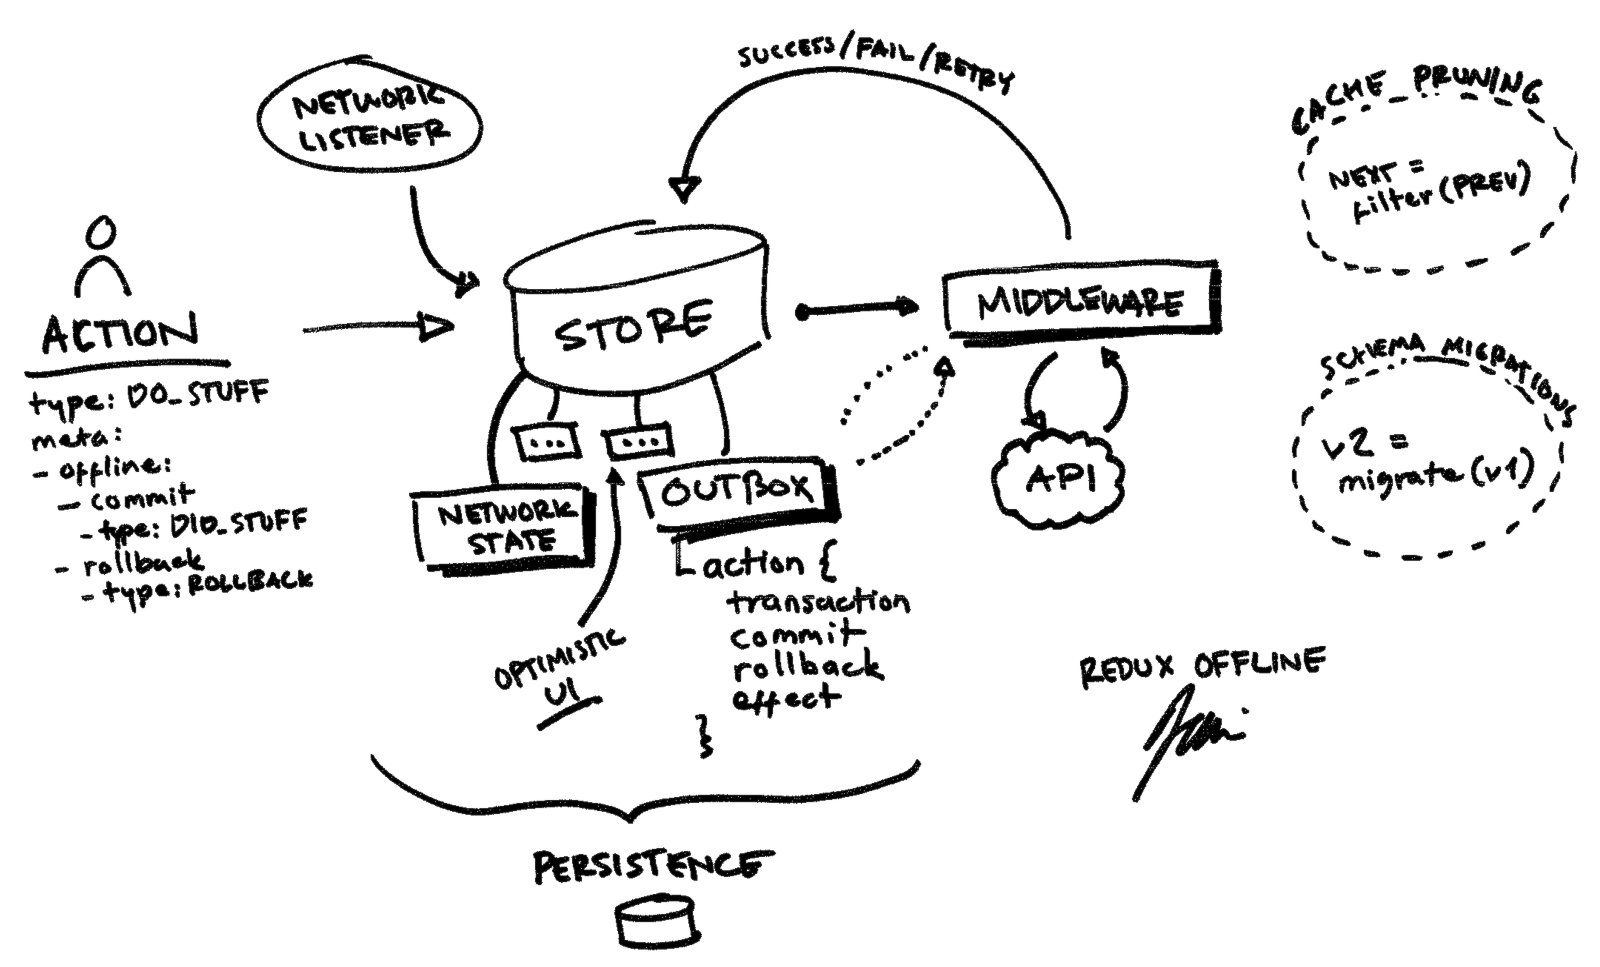
\includegraphics[width=\textwidth]{redux-offline}
  \grayRule
  \caption[Redux Offline]{Redux Offline Architektur\\\\~Quelle:~\cite{redux-offline}}
  \label{fig:redux-offline}
\end{figure}
Die grundlegende Idee hinter Redux Offline ist, dass der \sc{Redux store} die Datenbank ersetzt/ist. Jede Aktion die benötigt wird um offline zu arbeiten, wird im \sc{store} persisiert und durch die \tt{meta.offline} -Daten weiß die Anwendung was online zu tun ist. Wie die Grafik \ref{fig:redux-offline} (links) zeigt, wird jede (offline-unterstützende) Aktion mit dem \tt{offline.meta} Feld dekoriert. Darin wird beschrieben, wie der \it{Netzwerkeffekt} ausgeführt werden soll (\tt{effect}) und welche Aktion ausgelöst werden soll, wenn sie erfolgreich (\tt{commit}) ist oder fehlschlägt (\tt{rollback}). Diese Offline-Aktionen werden im \sc{store}-internen \gls{Queue} gespeichert und werden, einmal online, an den Server gesendet.\\\\
\gls{UI}\\
Es umfasst netzwerkfähige \gls{API}-Aufrufe, das Persistieren des Zustands(Status), das Stapeln von Nachrichten und die Behandlung von Fehlern, Neuversuchen, \gls{optimistic UI}-Aktualisierungen, Migrationen, Cache-Bereinigung und mehr.
Weil das kompliziert sein kann, zielt \sc{Redux Offline} darauf ab, eine vernünftige Reihe von Standardverhaltensweisen zu bieten, die verwendet werden, und nach Bedarf einzeln überschrieben werden können.\\
Grundsätzlich ist das Problem, das \sc{Redux Offline} löst, kein technisches, sondern ein Architekturproblem. Architekturen können im Code implementiert werden, aber um verstanden, angewendet und nachvollziehbar zu werden, müssen sie gut kommuniziert werden. --> Dokumentation

{\large Konflikte?}
%
% redux persist
%
\subsub{redux-persist}
localStorage. github~\cite{redux-persist-gh} medium~\cite{redux-persist}
\subsub{redux-optimist}

%
% react-native-offline
%
\sub{react-native-offline}
React Native = JavaScript React Framework um native, mobile Apps zu bauen. blabla\\
Behandelt online/offline Verbindung. Kann die Internetverbindung auch regelmäßig prüfen\\
Speichert nur den Status online/offline im store. -> erlaubt so unterschiedliches Rendern von Componenten.\\

\tt{const YourComponent = ({ isConnected }) => (\\
  <Text>{isConnected ? 'I am connected to the internet!' : 'Offline :('}</Text>\\
  );\\}\\
  Zusammen mir Redux hat es einen `Mehrwert`:
  Hat dann einen `Offline-\gls{Queue} um Aktionen zu wiederholen (im Intervall) \tt{meta.retry? \textcolor{gray}  {Array of actions which, once dispatched, will trigger a dismissal from the queue}} ~ oder nicht \tt{meta.dismiss? []}.\cite{rn-offline-gh}
  % \cite{rn-offline-medium}


%
% webpack offline-plugin
%
\sub{offline-plugin für webpack}
webpack ist ein JavaScript `Bundler`, packt JavaScript-Dateien und oder \gls{Assets} für die Verwendung in Browsern.blabla\\
Bietet offline experience für webpack Projekte. Benutzt \sc{ServiceWorker} und \sc{AppCache} unter der Haube --> cached nur (gebündelten) von webpack generierten \gls{Assets}. Für die anderen Dateien (z.B. index.html die nicht gebundled wird oder Modul von CDN) braucht mal ein \tt{html-plugin} oder benutzt die \tt{externals} :\\\\
\tt{const OfflinePlugin = require('offline-plugin')\\
  const offline = new OfflinePlugin\\\\
  const offline = new OfflinePlugin({\\
    externals: ['index.html'],\\
    })}\\
Es gibt diverse config-options für \sc{ServiceWorker} und AppCache...~\cite{webpack-gh}
% dev\cite{webpack-dev}


%
% hoodie
%
\sub{hoodie}
Benutzt CouchDB und PouchDB...\cite{hoodie}
%
% Couch
%
\subsub{\label{sec:couch}CouchDB}
Apache CouchDB\tm ist ein \gls{DBMS} das seit 2005 als freie Software entwickelt wird. Die dokumentenorientierte \gls{DB} funktioniert sowohl als einzelne Instanz, als auch im Cluster, in dem ein Datenbanksserver auf einer beliebig großen Anzahl an Servern oder \glspl{VM} ausgeführt werden kann. So kann die Datenschicht beliebig skaliert werden, um die Anforderungen vieler BenutzerInnen zu erfüllen. CouchDB verwendet das HTTP--Protokoll und \gls{JSON} als Datenformat, weswegen es mit jeder Software kompatibel ist, die das unterstützt.\\
Eine weitere Besonderheit ist das implementierte Replikationsmodell. Dessen Funktionsweise wird in \autoref{sec:replication} detailliert beschrieben. Dieses Protokoll ist die Grundlage für Offline First Anwendungen. So kann beispielsweise eine CouchDB-Instanz auf dem Mobiltelefon und eine auf dem Laptop bestehen und beide können sich bei bestehender Internetverbindung synchronisieren. Da so die gespeicherten Daten aus dem lokalen Speicher gelesen werden, sind ein schnelles Interface und eine geringe Latenz die positive Folge. Wenn Konflikte auftreten, beispielsweise durch gleichzeitiges Bearbeiten eines Dokuments von zwei Personen ohne Netzwerkverbindung, gehen keine Daten verloren und es liegt an der benutzenden Person diese zu lösen. CouchDB ist für Server konzipiert. Für Browser gibt es \hyperref[sub:pouch]{PouchDB} und für native iOS- und Android--\glspl{App} wurde \hyperref[sub:couchbase]{Couchbase Lite} entwickelt. Alle können Daten miteinander replizieren und verwenden das CouchDB Replikationsprotokoll.~\cite{couch}\\
\subsub{Replikation?}
\subsub{Eventual Consistency?}
%
% Pouch
%
\subsub{\label{sub:pouch}PouchDB}
Als Ergänzung zu CouchDB kann PouchDB verwendet werden. PouchDB ist eine Open--Source--JavaScript--Datenbank, die so konzipiert wurde, dass sie im Browser läuft. PouchDB ermöglicht es Anwendungen zu erstellen, die sowohl offline als auch online funktionieren. Daten können lokal gespeichert werden, sodass alle Funktionen der Anwendung auch im Offline--Modus zur Verfügung stehen.
Daten werden unabhängig von der nächsten Anmeldung (des nächsten Onlinezugangs) zwischen \b{Clients}, CouchDB oder kompatiblen Servern synchronisiert.
PouchDB läuft auch in Node.js\footnote{JavaScript Laufzeitumgebung, steht unter \url{https://nodejs.org/en/download/} zum Download bereit} und kann als direkte Schnittstelle zu CouchDB--kompatiblen Servern verwendet werden~\cite{pouch}.
\sub{\label{sub:couchbase}Couchbase}
